%% LaTeX template prepared by Sami Lewis for students in NE 101/210M, fall 2016
%% NOTES:
%%			- This is a simple, bare-bones template for the purposes of typing up homeworks. 
%%				There are many more advanced things you can add if you wish to do so.
%%			- You can make any changes to the template that you'd like.
%%			- Things in all caps are things you need to fill in. Make sure to change them
%%				all, including your name.
%%			-	There are lots of other, nicer free templates online too!
%%			- Run the template once without making any changes so that you can install
%%				all of the packages and see what the formatting looks like.

\documentclass{report}
% PACKAGES %
\usepackage[english]{} % Sets the language
\usepackage[margin=2cm]{geometry} % Sets the margin size
\usepackage{graphicx} % Enhanced package for including graphics/figures
\usepackage{float} % Allows figures and tables to be floats
\usepackage{amsmath} % Enhanced math package prepared by the American Mathematical Society
\usepackage{amssymb} % AMS symbols package
\usepackage{bm} % Allows you to use \bm{} to make any symbol bold
\usepackage{verbatim} % Allows you to include code snippets
\usepackage{setspace} % Allows you to change the spacing between lines at different points in the document
\usepackage{parskip} % Allows you alter the spacing between paragraphs
\usepackage{multicol} % Allows text division into multiple columns
\usepackage{units} % Allows fractions to be expressed diagonally instead of vertically
\usepackage{booktabs,multirow,multirow} % Gives extra table functionality
\usepackage{enumerate}
\newcommand{\tab}{\-\hspace{1.5cm}}

% Set path to figure image files
\graphicspath{ {fig/} }

\begin{document}

\begin{center}
\textbf{\large Nuclear Engineering 150 -- Discussion Section}\\ 
\textbf{Team Exercises \#1}

\-\\
{\small *Problems 1 \& 2 borrowed from Nuclear Engineering 101 homework problem sets, Fall 2016}
\end{center}

%%%%%%%%%%%%%%%%%%%%%%%%%%%%%%%%%% PROBLEM 1 %%%%%%%%%%%%%%%%%%%%%%%%%%%%%%%%%%
\section*{Problem 1}
The radioactive isotope $^{233}$Pa can be produced following neutron capture by $^{232}$Th when the resulting $^{233}$Th decays to $^{233}$Pa. In the neutron flux of a typical reactor, neutron capture in 1 g of $^{232}$Th produces $^{233}$Th at of a rate of $2.0 \times 10^{11}\text{ s}^{-1}$.
\begin{enumerate}[a)]
\item What are the activities (in Ci) of $^{233}$Th and $^{233}$Pa after this sample is irradiated for 1.5 hours?
\item The sample is then placed in storage with no further irradiation so that the $^{233}$Th can decay away. What are
the activities (in Ci) of $^{233}$Th and $^{233}$Pa after 48 hours of storage?
\item The decay of $^{233}$Pa results in $^{233}$U, which is also radioactive. After the above sample has been stored for 1 year what is the $^{233}$U activity in Ci? (Hint: it should not be necessary to set up an additional differential equation to find the $^{233}$U activity.)
\end{enumerate}

\begin{table}[htbp]
	\centering
	\begin{tabular}{|c|c|}
			\hline
			Nucleus		&	Half-life \\
			\hline
			$^{233}$Th	&  $22.3$ min\\
			$^{233}$Pa	&  $27.0$ days\\
			$^{233}$U	&  $1.592 \times 10^5$ yr\\
			\hline
	\end{tabular}
	\label{tab:design-specs}
\end{table}
\begin{center}$1\text{ Ci} = 3.7 \times 10^{10}\text{ s}^{-1}$\end{center}



\newpage
%%%%%%%%%%%%%%%%%%%%%%%%%%%%%%%%%% PROBLEM 2 %%%%%%%%%%%%%%%%%%%%%%%%%%%%%%%%%%
\section*{Problem 2}

Use the following masses for parts (a) and (b):

\begin{table}[htbp]
	\centering
	\begin{tabular}{|c|c|}
			\hline
			Nucleus		&	Atomic Mass \\
			\hline
			n 			&	 1.008665 u \\
			$^{1}$H		& 	 1.007825 u \\
			$^{2}$H 	&	 2.014102 u \\
			$^{56}$Fe	&   55.934939 u \\
			$^{98}$Y 	&   97.922203 u \\
			$^{135}$I	&  134.910048 u \\
			$^{235}$U	&  235.043924 u \\
			\hline
	\end{tabular}
	\label{tab:design-specs}
\end{table}
\begin{center}$1\text{u} \cdot c^{2} = 931.502$ MeV\end{center}
\-\\
\-\\
\begin{enumerate}[a)]
\item Calculate the $Q$-value of the reaction:
$$ ^{235}\text{U}\, + \,n \-\rightarrow\- ^{135}\text{I}\, + \,^{98}\text{Y}\, + \,3n $$
\item Calculate the average binding energy per nucleon (in MeV) of $^{2}$H, $^{56}$Fe, and $^{235}$U.

\end{enumerate}



\newpage
%%%%%%%%%%%%%%%%%%%%%%%%%%%%%%%%%% PROBLEM 3 %%%%%%%%%%%%%%%%%%%%%%%%%%%%%%%%%%
\section*{Problem 3}

\begin{enumerate}[a)]
\item Solve the first order differential equation
$$ \frac{dy}{dx} + 3y = 0 $$
\item Solve the second order differential equation ($A$ and $B$ are constants)
$$ \frac{d^2 y}{dx^2} - A^2y = B $$
The boundary condition is $y(\pm\frac{1}{A}) = 0$.
\end{enumerate}



\newpage
%%%%%%%%%%%%%%%%%%%%%%%%%%%%%%%%%% PROBLEM 4 %%%%%%%%%%%%%%%%%%%%%%%%%%%%%%%%%%
\section*{Problem 4}

Classify the following cross section plots. They are, in no particular order:
\begin{enumerate}[(1)]
\item $^{155}$Gd absorption
\item $^{235}$U fission
\item $^{238}$U absorption
\item $^{238}$U fission
\item $^{239}$Pu fission
\end{enumerate}

\begin{center}
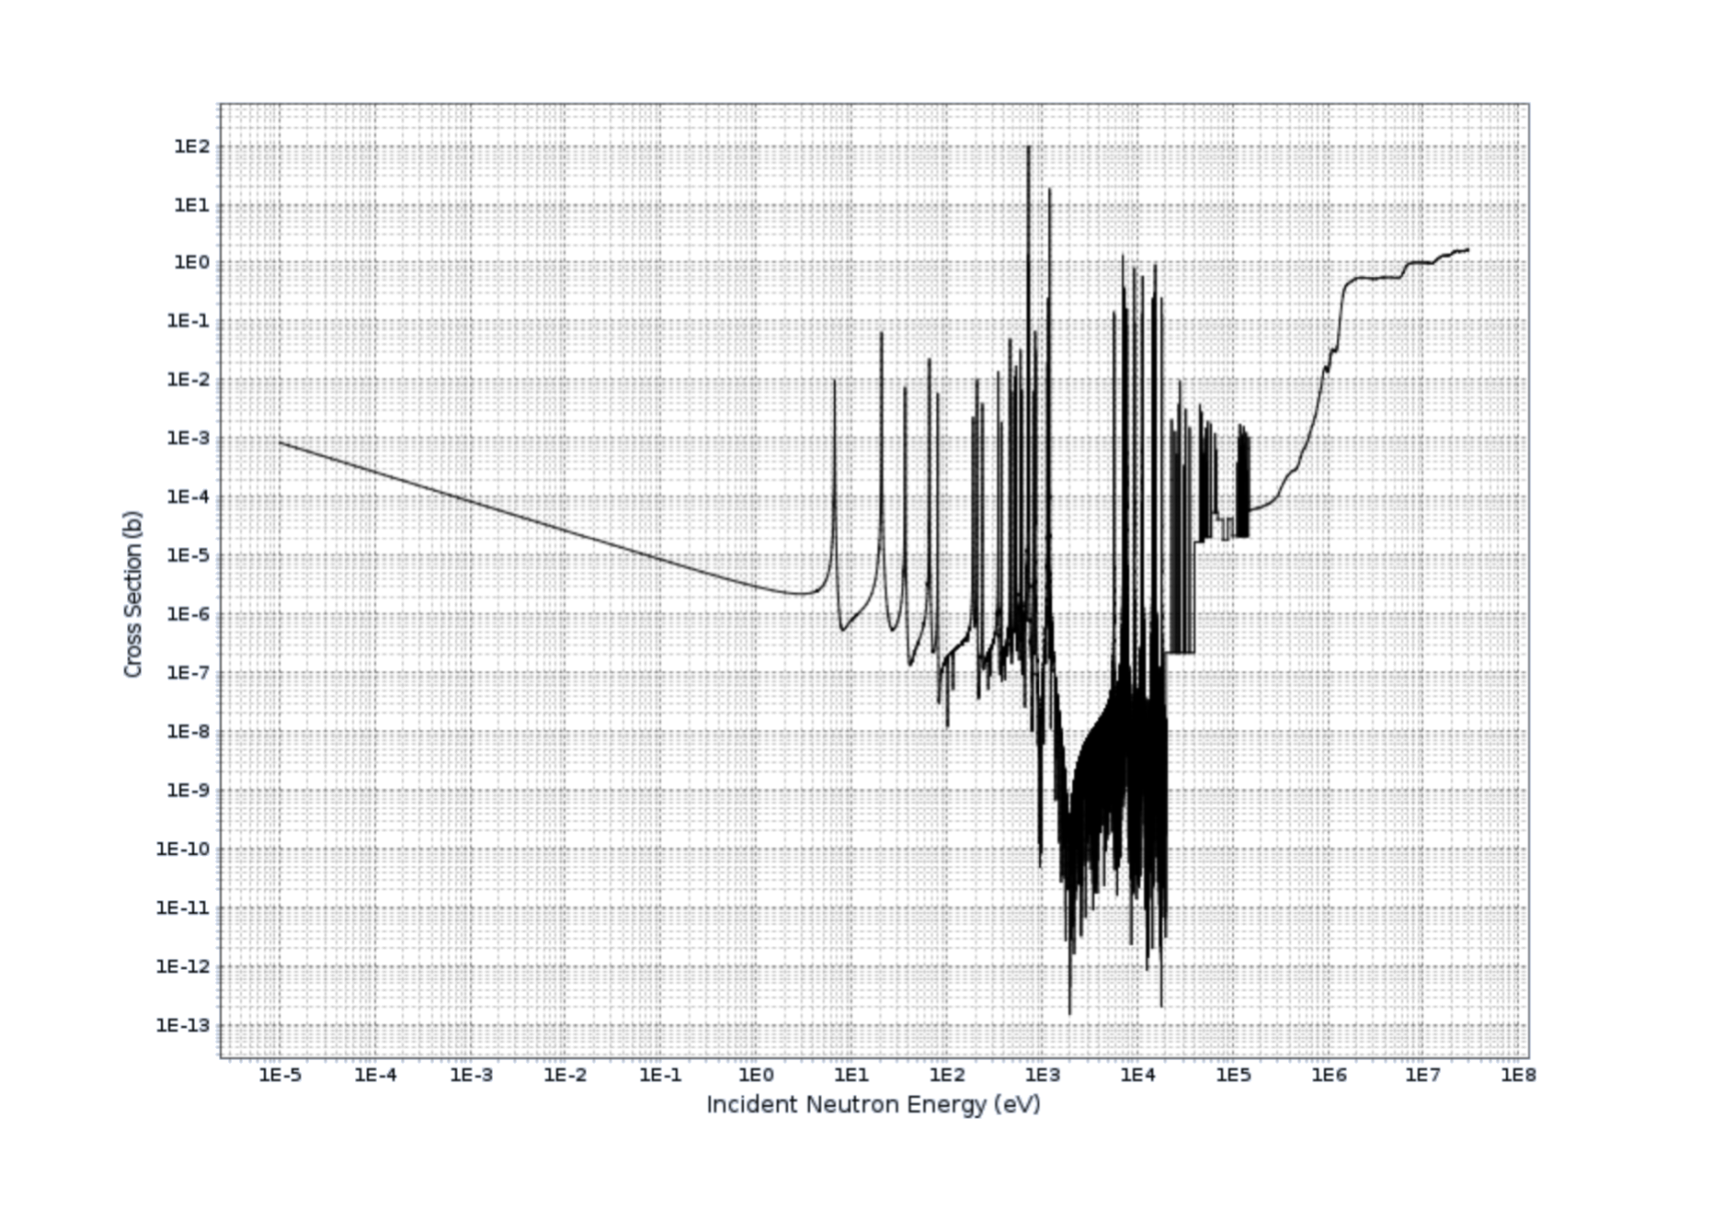
\includegraphics[width=11cm]{u238_fission.png}\\
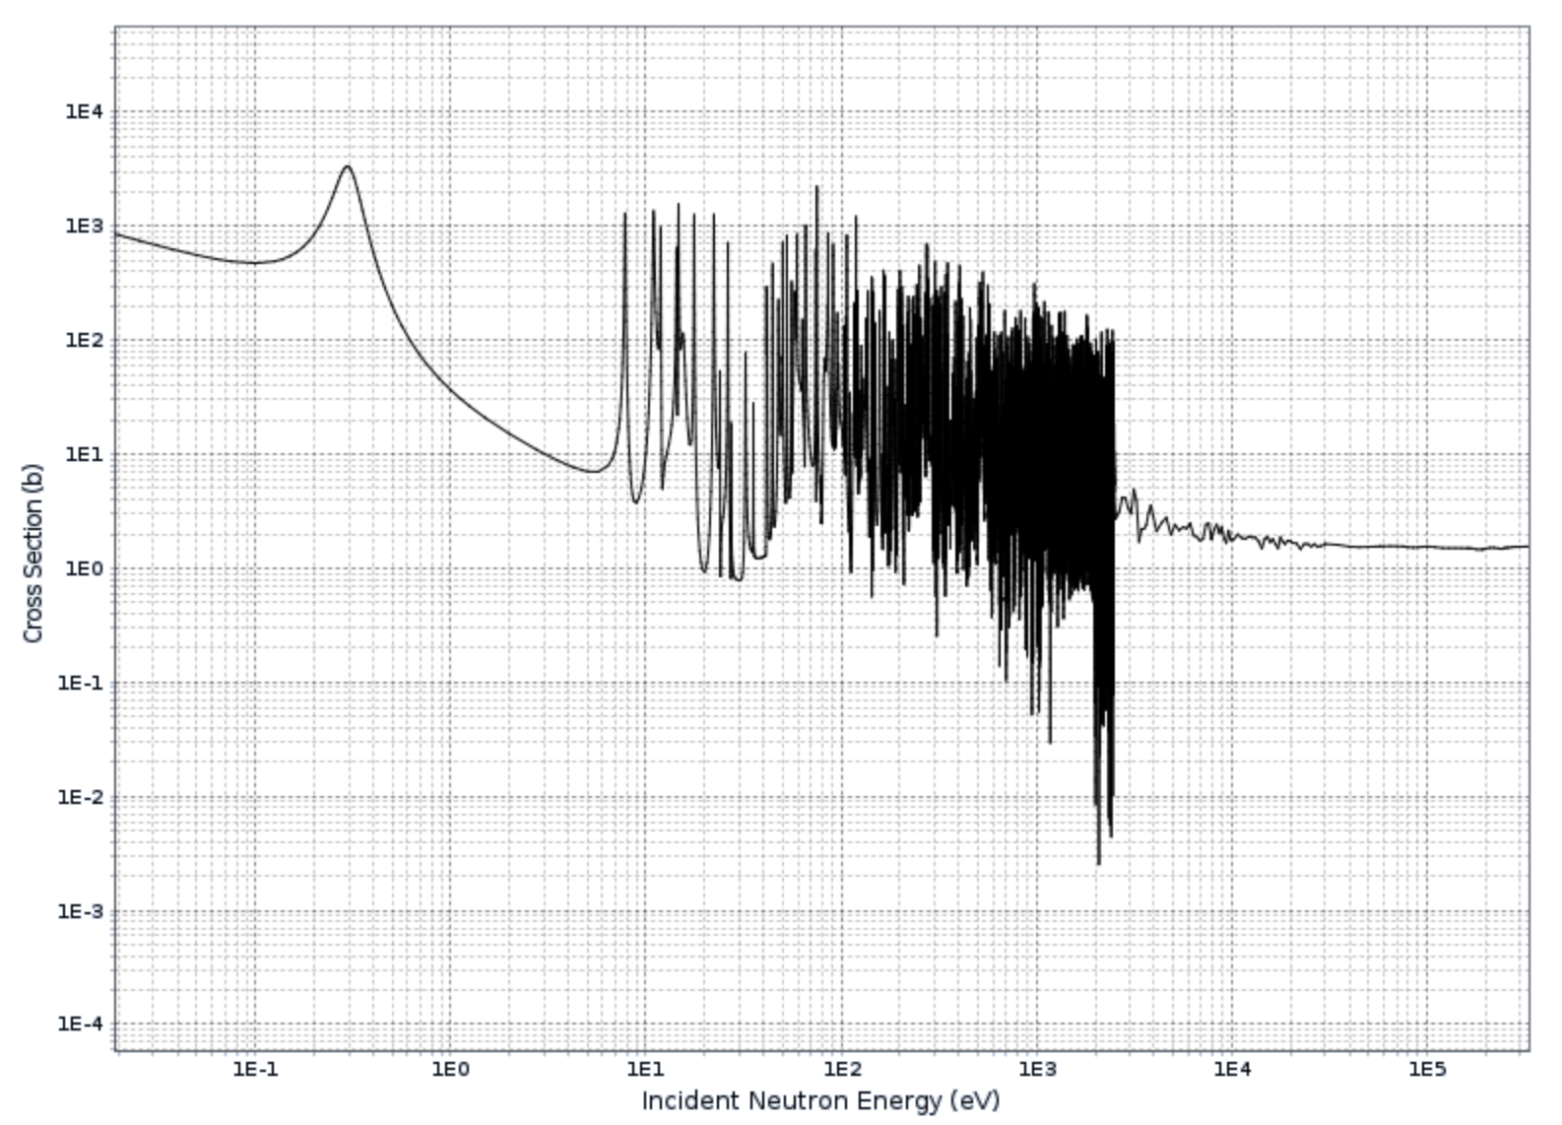
\includegraphics[width=11cm]{pu239_fission.png}\\
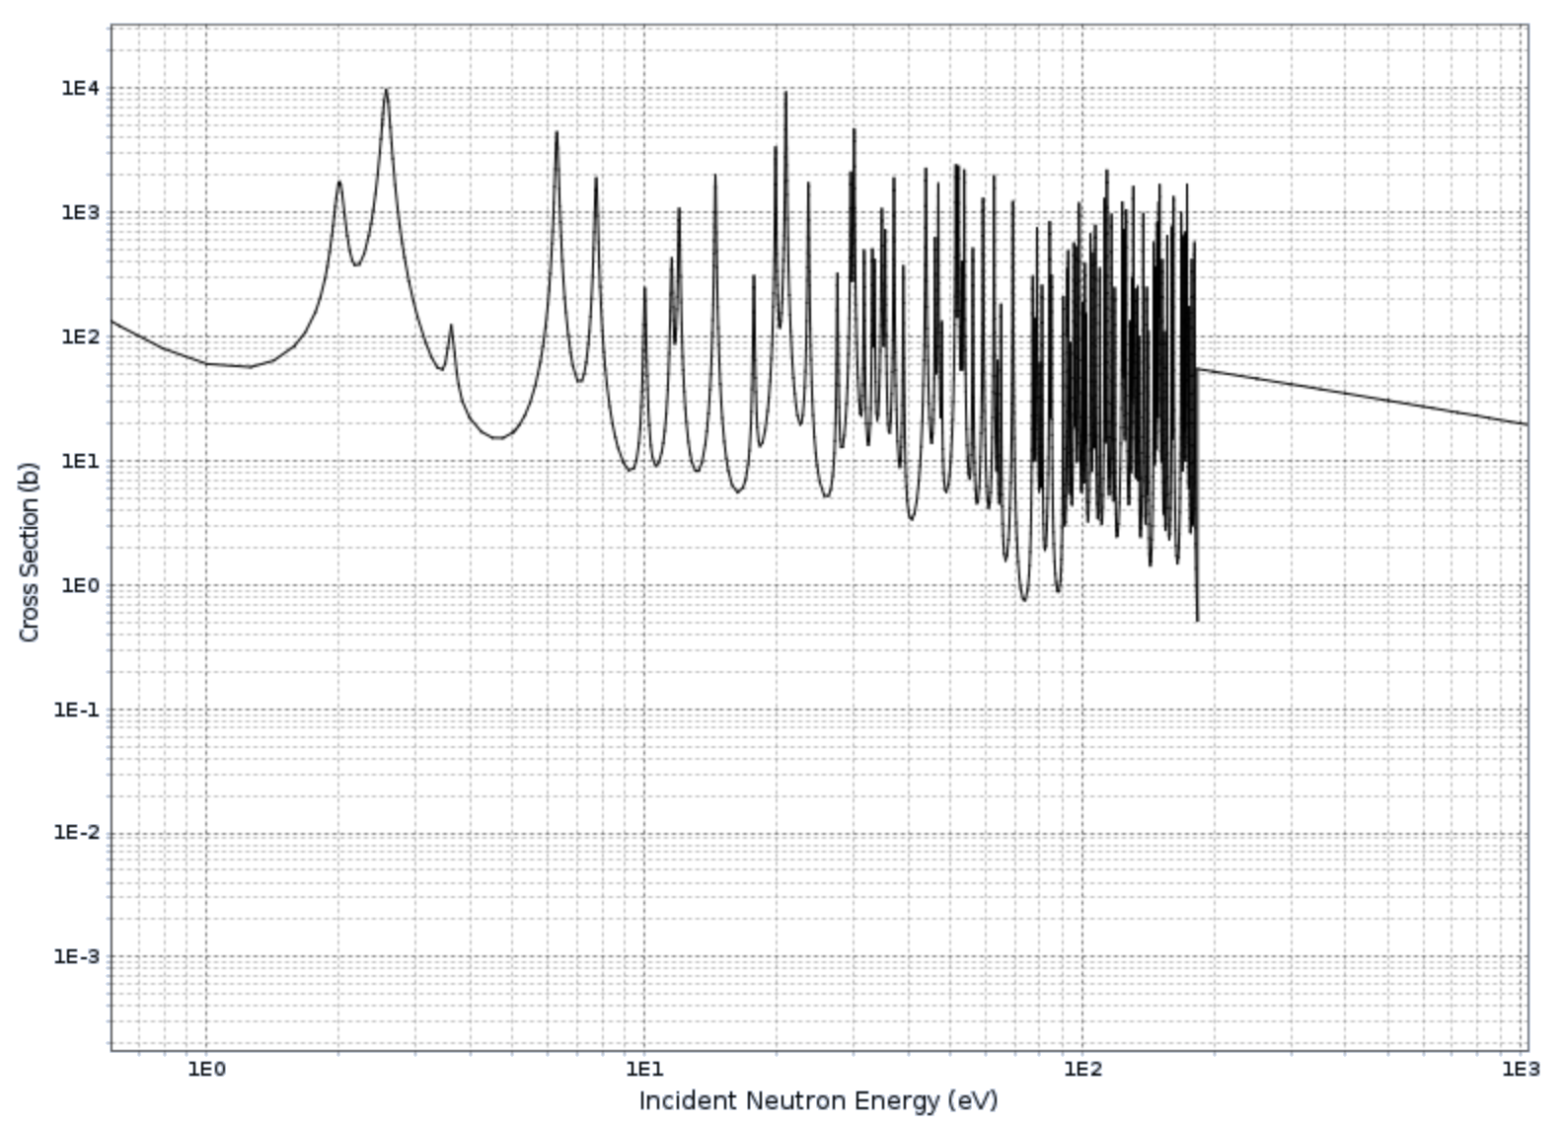
\includegraphics[width=11cm]{gd155_absorption.png}\\
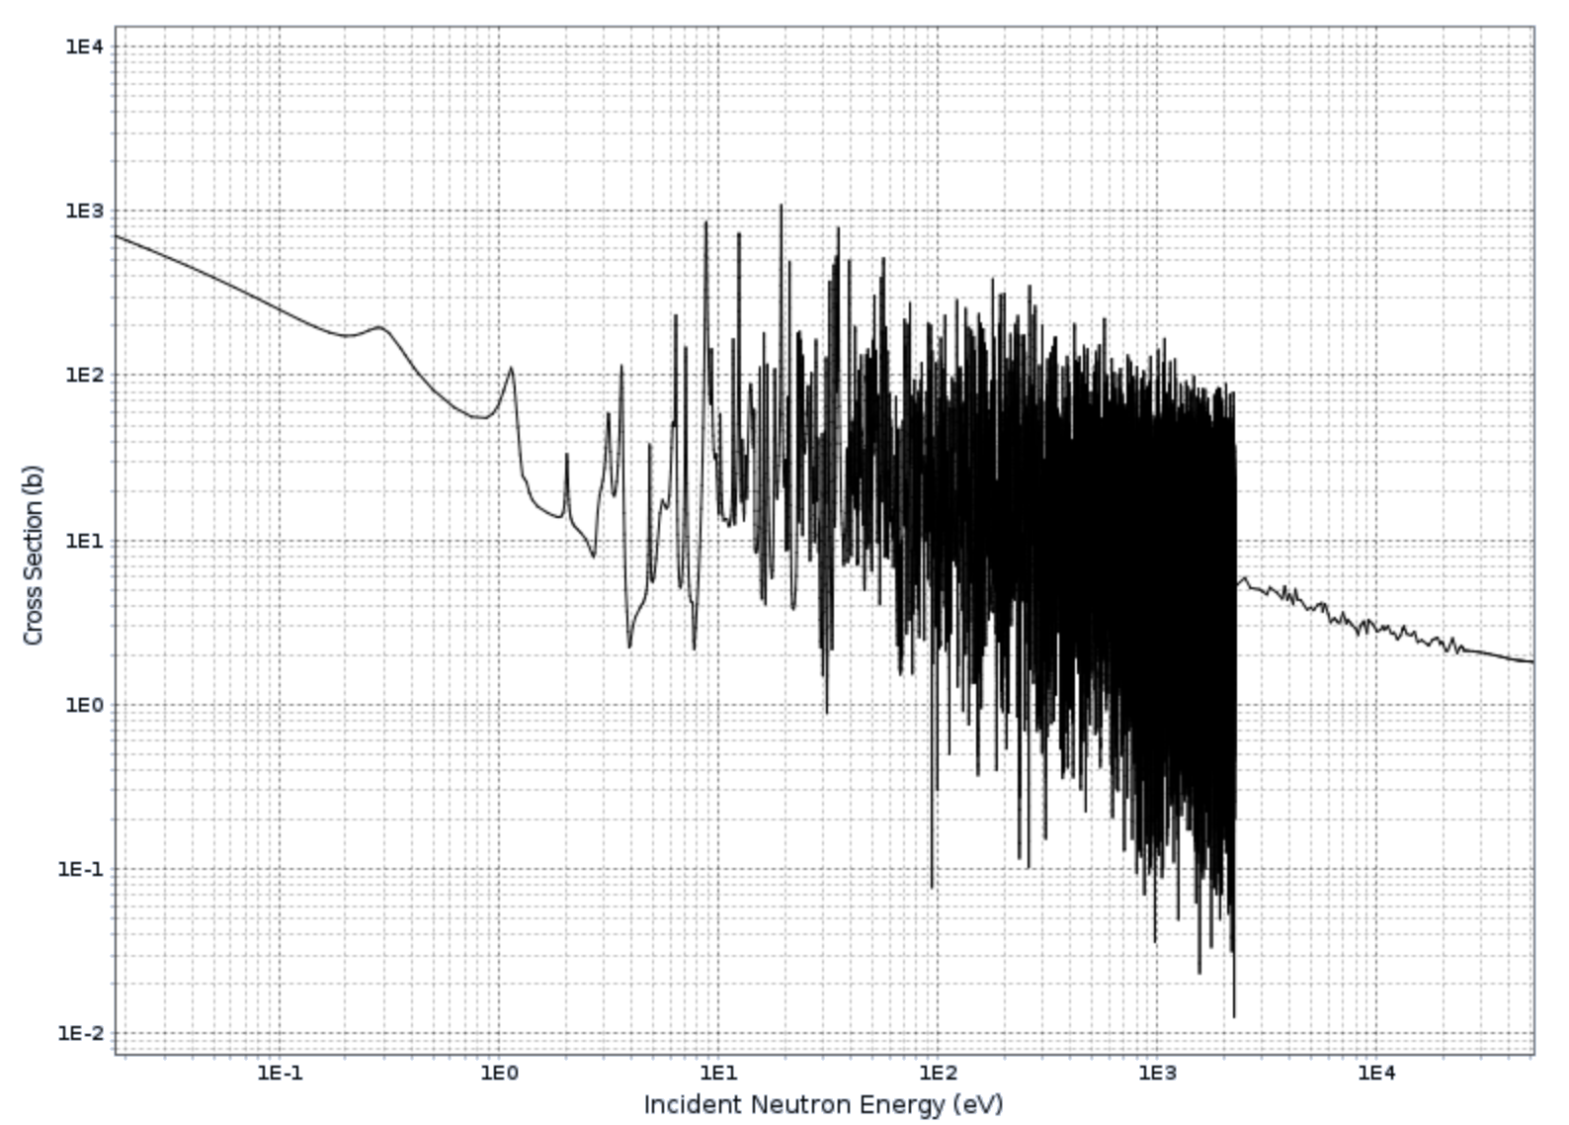
\includegraphics[width=11cm]{u235_fission.png}\\
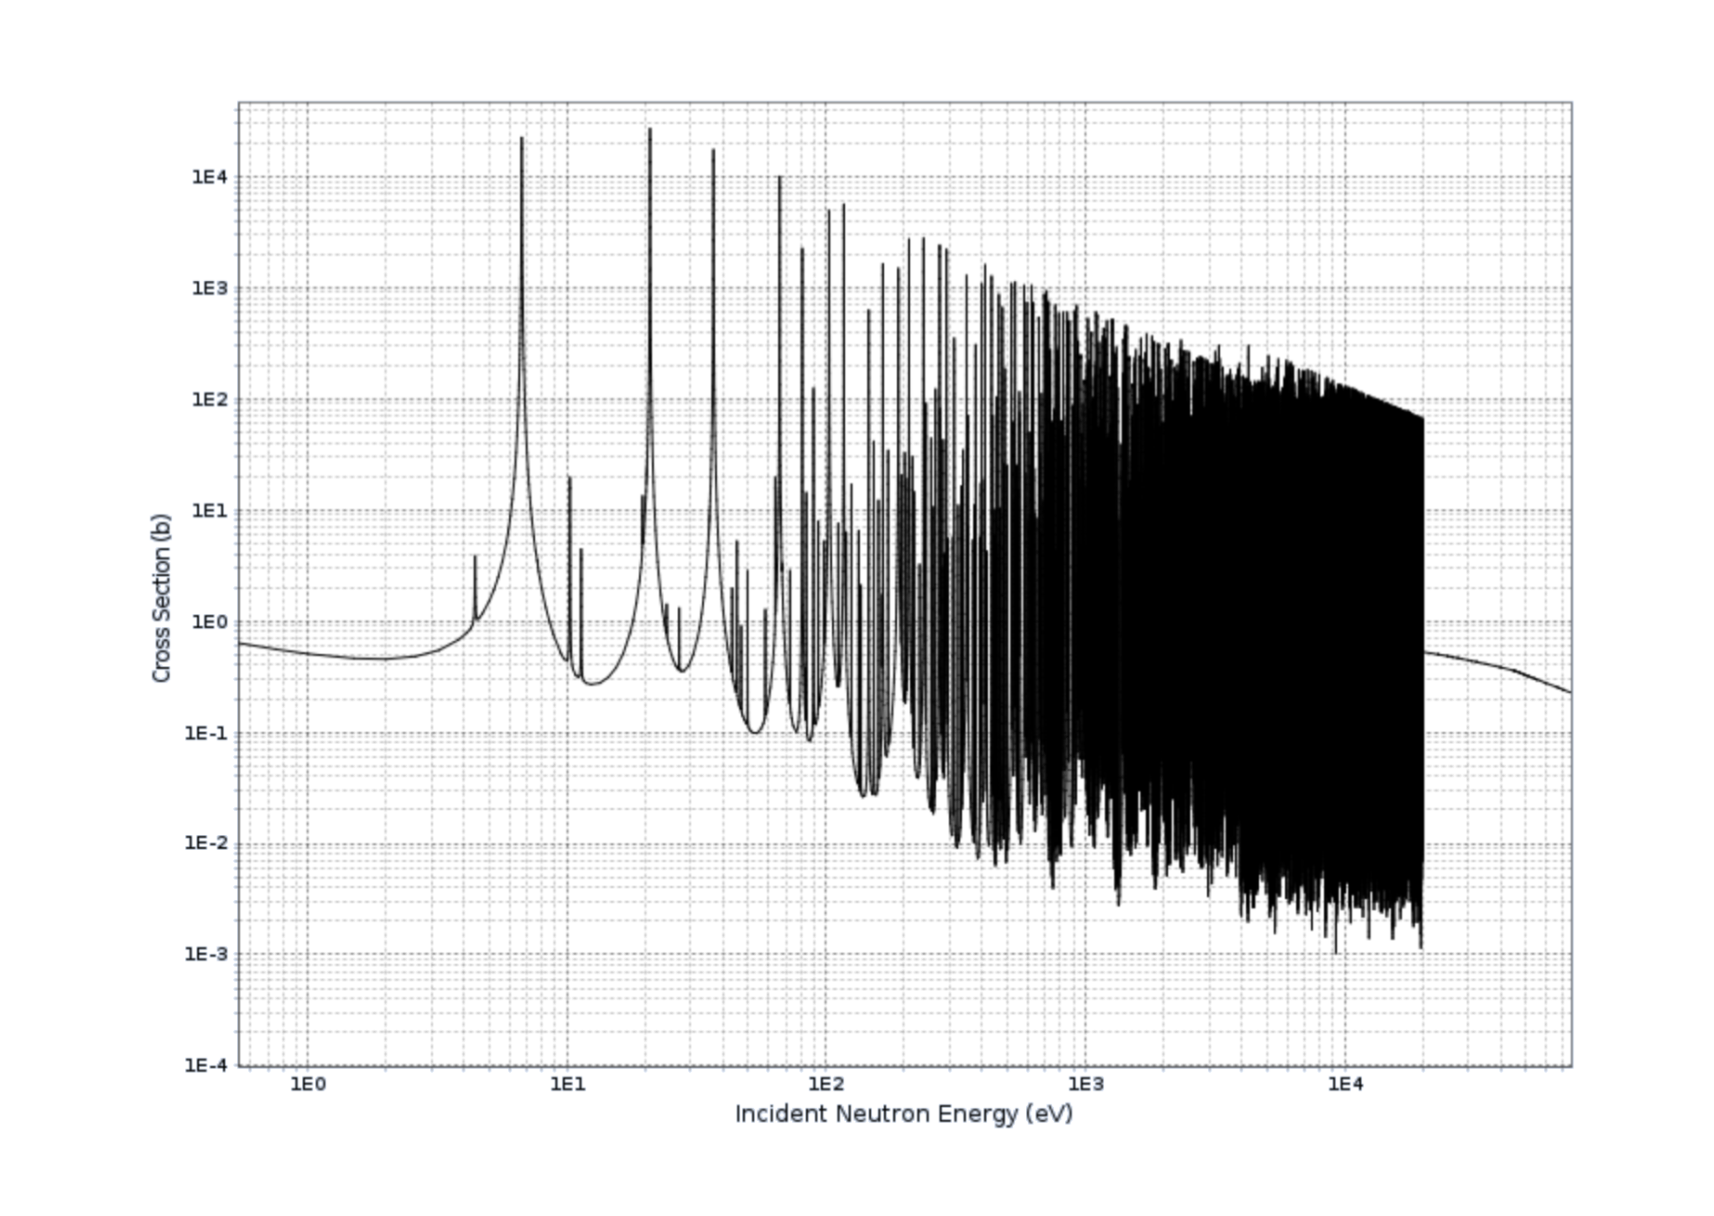
\includegraphics[width=11cm]{u238_absorption.png}\\
\end{center}



\end{document}

